\section{Producción}\label{docProduccion}
La segunda etapa en Hundle es la producción. Esta estapa se encarga de asegurarse que que el proceso se siga, que los artefactos esten al día y que el equipo trabaje. Se debe estar al pendiente de los requerimienos especificados y las características nuevas que puedan agregarse. Consta de los detalles del proyecto, sprint plan, project chart, feature log, sprint backlog, task chart, burn-down chart, buglist y task slips. 

\subsection{Detalles del proyecto}
Aquí se mostrará del proyecto el título, estudio, género, plataforma, fecha de inicio, fecha de término, lo planeado, en desarrollo, sin planear y terminado.
\\
\subsubsection{Título}
Yolotl

\subsubsection{Estudio}
ESCOM - IPN

\subsubsection{Plataforma}
Dispositivos móviles android

\subsubsection{Fecha de inicio}
1 Agosto 2017

\subsubsection{Fecha de término}
1 Junio 2018
\subsubsection{Planeado}
El 80\%
\subsubsection{Desarrollo}
El 10\%
\subsubsection{Planear}
El 20\%
\subsubsection{Terminado}
El 0\%



\subsection{Sprint plan 1}
\subsubsection{SprintID}
01
\subsubsection{Inicio}
1 Agosto 2017
\subsubsection{Fin}
31 Agosto 2017
\subsubsection{Meta}
Nivel 1
\subsubsection{Porcentaje}
El 16\% 


\subsubsection{FeatureID}
01
\subsubsection{Nombre}
N1
\subsubsection{Estado}
Planeado

\subsubsection{SprintID}
01
\subsubsection{Comentarios}
-


\subsection{Sprint backlog 1}
\subsubsection{Sprint backlog}
01

\subsubsection{Tareas}
6
\subsubsection{Tendencia}
0
\subsubsection{Esfuerzo restante}
56
\subsubsection{Tendencia actual}
-
\subsubsection{Progreso ideal}
10
\subsubsection{Tareas restantes}
10
\subsubsection{Nombre de la tarea}
n1
\subsubsection{FeatureID}
01
\subsubsection{Miembro}
Rocío
\subsubsection{Rol}
Desarrollo
\subsubsection{Estado}
Planeado
\subsubsection{Esfuerzo}
10
\subsection{Buglist}
\subsubsection{BugID}
01
\subsubsection{Descripción}
Doble salto infinito
\subsubsection{Descripción técnica}
El gameobject no realiza la función detectar colisión de el "piso" 
\subsubsection{Autor}
Velez
\subsubsection{Estado}
Revisión
\subsubsection{FeatureID}
01


\subsection{Task Slips 1}


\subsubsection{FeatureID}1
\subsubsection{Nombre}Maqueta
\subsubsection{Tarea}Realizar maqueta del nivel completo
\subsubsection{Miembro}Rocío
\subsubsection{Esfuerzo estimado}1
\subsubsection{Terminado}si
\subsubsection{Restante}0


\subsubsection{FeatureID} 1
\subsubsection{Nombre} Enemigos
\subsubsection{Tarea} Realizar el comportamiento de los enemigos o cualquier otra acción necesaria dentro del nivel
\subsubsection{Miembro} Rocio
\subsubsection{Esfuerzo estimado} 3
\subsubsection{Terminado} sí
\subsubsection{Restante} 0


\subsubsection{FeatureID} 1
\subsubsection{Nombre} Arte 1
\subsubsection{Tarea} Crear vista de los personajes
\subsubsection{Miembro} Rocío
\subsubsection{Esfuerzo estimado} 2
\subsubsection{Terminado} sí
\subsubsection{Restante} 0



\subsubsection{FeatureID} 1
\subsubsection{Nombre} Arte 2
\subsubsection{Tarea} Crear el diseño de los obstáculos
\subsubsection{Miembro} Rocío
\subsubsection{Esfuerzo estimado} 2
\subsubsection{Terminado} sí
\subsubsection{Restante} 0


\subsubsection{FeatureID} 1
\subsubsection{Nombre} Arte 3
\subsubsection{Tarea} Crear el diseño de los items
\subsubsection{Miembro} Rocio
\subsubsection{Esfuerzo estimado} 2
\subsubsection{Terminado} sí
\subsubsection{Restante} 0


\subsection{Sprint plan 3}
\subsubsection{SprintID}
03
\subsubsection{Inicio}
25 Septiembre 2017
\subsubsection{Fin}
24 Diciembre 2017
\subsubsection{Meta}
Nivel 2
\subsubsection{Porcentaje}
El 16\% 

\subsubsection{FeatureID}
03
\subsubsection{Nombre}
N3
\subsubsection{Estado}
Planeado
\subsubsection{SprintID}
03
\subsubsection{Comentarios}
-


\subsection{Sprint backlog 3}
\subsubsection{Sprint backlog}
03

\subsubsection{Tareas}
14
\subsubsection{Tendencia}
0
\subsubsection{Esfuerzo restante}
56
\subsubsection{Tendencia actual}
-
\subsubsection{Progreso ideal}
14
\subsubsection{Tareas restantes}
14
\subsubsection{Nombre de la tarea}
n3
\subsubsection{FeatureID}
03
\subsubsection{Miembro}
Rocío
\subsubsection{Rol}
Desarrollo
\subsubsection{Estado}
Planeado
\subsubsection{Esfuerzo}
14

\subsection{Task Slips 3}


\subsubsection{FeatureID}3
\subsubsection{Nombre}Maqueta
\subsubsection{Tarea}Realizar maqueta del nivel completo
\subsubsection{Miembro}Rocío
\subsubsection{Esfuerzo estimado}1
\subsubsection{Terminado}si
\subsubsection{Restante}0


\subsubsection{FeatureID} 3
\subsubsection{Nombre} Enemigos
\subsubsection{Tarea} Realizar el comportamiento de los enemigos o cualquier otra acción necesaria dentro del nivel
\subsubsection{Miembro} Rocio
\subsubsection{Esfuerzo estimado} 3
\subsubsection{Terminado} sí
\subsubsection{Restante} 0


\subsubsection{FeatureID} 3
\subsubsection{Nombre} Arte 1
\subsubsection{Tarea} Crear vista de los personajes
\subsubsection{Miembro} Rocío
\subsubsection{Esfuerzo estimado} 2
\subsubsection{Terminado} sí
\subsubsection{Restante} 0



\subsubsection{FeatureID} 3
\subsubsection{Nombre} Arte 2
\subsubsection{Tarea} Crear el diseño de los obstáculos
\subsubsection{Miembro} Rocío
\subsubsection{Esfuerzo estimado} 2
\subsubsection{Terminado} sí
\subsubsection{Restante} 0


\subsubsection{FeatureID} 3
\subsubsection{Nombre} Arte 3
\subsubsection{Tarea} Crear el diseño de los items
\subsubsection{Miembro} Rocio
\subsubsection{Esfuerzo estimado} 2
\subsubsection{Terminado} sí
\subsubsection{Restante} 0

\subsubsection{FeatureID} 3
\subsubsection{Nombre} Boss 1
\subsubsection{Tarea} Diseñar la máquina de estados del enemigo principal del nivel
\subsubsection{Miembro} Rocio
\subsubsection{Esfuerzo estimado} 2
\subsubsection{Terminado} sí
\subsubsection{Restante} 0

\subsubsection{FeatureID} 3
\subsubsection{Nombre} Boss 2
\subsubsection{Tarea} Crear la máquina de estados del enemigo principal del nivel
\subsubsection{Miembro} Rocio
\subsubsection{Esfuerzo estimado} 2
\subsubsection{Terminado} sí
\subsubsection{Restante} 0



\section{Quinto sprint de producción}

Esta etapa contiene el desarrollo del nivel quinto del juego. El panorama general abarca un nivel de manera ascendente en un terreno nevoso. Después se llega al jefe enemigo Mictlecayotl.

Primero se empieza con el maquetado del nivel, para establecer el tamaño del nivel, nuevamente es de manera vertical el diseño, y la cámara solo se moverá en esa dirección. Se establece también donde debe ir cada objeto o enemigo junto con anotaciones necesarias para la comprensión posterior, como son direcciones de movimiento o acciones que deben realizarse. Recordando que se debe tomar muy en cuenta el tamaño del personaje a jugar si no, no se podrá avanzar en el nivel ya que se da la situación a atorarse debido al tamaño, incluido el espacio para saltar. Lo anterior se puede ver en la figura \ref{fig:n501}.
\begin{figure}[htbp]
	\centering
	\subfigure[Primera parte del nivel]{\includegraphics[width=5cm]{03TrabajoRealizado/DocProduccionR/imagenes/n5/06.jpeg}}
	\subfigure[Segunda parte del nivel]{\includegraphics[width=5cm]{03TrabajoRealizado/DocProduccionR/imagenes/n5/07.jpeg}}
	\subfigure[Tercera parte del nivel]{\includegraphics[width=5cm]{03TrabajoRealizado/DocProduccionR/imagenes/n5/08.jpeg}}
	\subfigure[Cuarta parte del nivel]{\includegraphics[width=5cm]{03TrabajoRealizado/DocProduccionR/imagenes/n5/09.jpeg}}
	\subfigure[Quinta parte del nivel]{\includegraphics[width=5cm]{03TrabajoRealizado/DocProduccionR/imagenes/n5/10.jpeg}}
	\caption{Maquetado de nivel cinco} \label{fig:n501}
\end{figure}  

Después se lleva la tarea de tomar todos los componentes solo de manera visual y adecuar el tamaño necesario, tomando en cuenta las medidas de los componentes anteriores. Dichas imágenes se pueden ver en la \ref{fig:n502}.
\begin{figure}[htbp]
	\centering
	\subfigure[Imagen de viento congelante.]{\includegraphics[width=5cm]{03TrabajoRealizado/DocProduccionR/imagenes/n5/n502.png}}
	\subfigure[Imagen de ave de nieve como enemigo.]{\includegraphics[width=5cm]{03TrabajoRealizado/DocProduccionR/imagenes/n5/n503.png}}
	\subfigure[Imagen de jefe enemigo Mictlecayotl]{\includegraphics[width=5cm]{03TrabajoRealizado/DocProduccionR/imagenes/n5/n504.png}}
	\subfigure[Imagen de tornado.]{\includegraphics[width=5cm]{03TrabajoRealizado/DocProduccionR/imagenes/n5/n505.png}}
	\subfigure[Imagen de cara de jefe enemigo]{\includegraphics[width=5cm]{03TrabajoRealizado/DocProduccionR/imagenes/n5/n506.png}}
	\subfigure[Imagen de terreno.]{\includegraphics[width=5cm]{03TrabajoRealizado/DocProduccionR/imagenes/n5/n510.png}}
	\caption{Imágenes utilizadas para el nivel} \label{fig:n502}
\end{figure}

Después de reunir los componentes se da a la tarea de dar las acciones que realizarían descritas dentro de la figura \ref{fig:n503}. En esta parte se omite las plataformas con movimiento tanto horizontal como vertical, pues presentan el mismo comportamiento que los anteriores. También se omite los enemigos fantasmas que ya han sido realizado en los niveles anteriores.
\begin{figure}[htbp]
	\centering
	\subfigure[Detección de pase de personaje por zona determinada, donde luego la bola de nieve caerá, pero esta al final de cierto tiempo desaparecerá.]{\includegraphics[width=5cm]{03TrabajoRealizado/DocProduccionR/imagenes/n5/n507.png}}
	\subfigure[Piso que desaparece despues de tocarlo simulando que se derrite, después de un tiempo establecido vuelve a aparecer.]{\includegraphics[width=5cm]{03TrabajoRealizado/DocProduccionR/imagenes/n5/n508.png}}
	\subfigure[Piso congelado que al ser tocado por el jugador simula que puede resbalarse sobre él.]{\includegraphics[width=5cm]{03TrabajoRealizado/DocProduccionR/imagenes/n5/n509.png}}
	\caption{Muestra de comportamiento de objetos} \label{fig:n503}
\end{figure}

Ya que se tiene los objetos con los comportamientos deseados se procede a ubicarlos según correspondan como se ve en la \ref{fig:n504}.
\begin{figure}
	\centering
	\caption{Maquetado llevado al motor de juego Unity.}
	\label{fig:n504}
	\includegraphics[width=0.5\textwidth]{03TrabajoRealizado/DocProduccionR/imagenes/n5/n501.png}
\end{figure}

Por último se establece las acciones que realiza el jefe enemigo Mictlecayotl descritas en la siguiente figura \ref{fig:n505}.
\begin{figure}[htbp]
	\centering
	\subfigure[El enemigo lanza de manera aleatoria hacia la izquierda o derecha un viento congelante.]{\includegraphics[width=5cm]{03TrabajoRealizado/DocProduccionR/imagenes/n5/n511.png}}
	\subfigure[El enemigo aparece de forma aleatoria por el eje horizontal sobre la superficie pequeños tornados.]{\includegraphics[width=5cm]{03TrabajoRealizado/DocProduccionR/imagenes/n5/n512.png}}
	\caption{Muestra de acciones de el jefe enemigo Mictlecayotl} \label{fig:n505}
\end{figure}


\subsection{Séptimo sprint de producción}

Esta etapa contiene el desarrollo del nivel séptimo del juego. El panorama general abarca un nivel de manera horizontal en un terreno arenoso. Después se llega al jefe enemigo Itztlacoliuhqui.

Primero se empieza con el maquetado del nivel, para establecer el tamaño del nivel, nuevamente es de manera vertical el diseño, y la cámara solo se moverá en esa dirección. Se establece también donde debe ir cada objeto o enemigo junto con anotaciones necesarias para la comprensión posterior, como son direcciones de movimiento o acciones que deben realizarse. Lo anterior se puede ver en la figura \cite{fig:n701}.
\begin{figure}[htbp]
	\centering
	\subfigure[Primera parte del nivel]{\includegraphics[width=5cm]{03TrabajoRealizado/DocProduccionR/imagenes/n7/11.png}}
	\subfigure[Segunda parte del nivel]{\includegraphics[width=5cm]{03TrabajoRealizado/DocProduccionR/imagenes/n7/12.png}}
	\caption{Maquetado de nivel siete} \label{fig:n701}
\end{figure}  

Después se lleva la tarea de tomar todos los componentes solo de manera visual y adecuar el tamaño necesario, tomando en cuenta las medidas de los componentes anteriores. Dichas imágenes se pueden ver en la \cite{fig:n702}.
\begin{figure}[htbp]
	\centering
	\subfigure[Imagen jefe enemigo Itztlacoliuhqui.]{\includegraphics[width=5cm]{03TrabajoRealizado/DocProduccionR/imagenes/n7/n702.png}}
	\subfigure[Imagen de flecha de obsidiana.]{\includegraphics[width=5cm]{03TrabajoRealizado/DocProduccionR/imagenes/n7/n703.png}}
	\subfigure[Imagen de fuego.]{\includegraphics[width=5cm]{03TrabajoRealizado/DocProduccionR/imagenes/n7/n704.png}}
	\subfigure[Imagen de mano gigante.]{\includegraphics[width=5cm]{03TrabajoRealizado/DocProduccionR/imagenes/n7/n705.png}}
	\caption{Imágenes utilizadas para el nivel} \label{fig:n702}
\end{figure}

Después de reunir los componentes se da a la tarea de dar las acciones que realizarían descritas dentro de la figura \cite{fig:n703}. En esta parte se omitirá las plataformas con movimiento tanto horizontal como vertical, pues presentan el mismo comportamiento que los anteriores. También se omite los enemigos fantasmas mostrados en niveles anteriores. Dejando solo la interacción de una lluvia constante de flechas de obsidiana, para que el nivel no fuera sobre cargado, se determino que solo la lluvia se efectuara a una distancia horizontal del jugador a cierto tiempo y desapareciendo al choque con cualquier objeto por parte de la flecha.
\begin{figure}[htbp]
	\centering
	\subfigure[Caída constante de flechas de obsidiana a lo largo del nivel de plataforma.]{\includegraphics[width=5cm]{03TrabajoRealizado/DocProduccionR/imagenes/n7/n709.png}}
	\caption{Muestra de comportamiento de objetos} \label{fig:n703}
\end{figure}

Ya que se tiene los objetos con los comportamientos deseados se procede a ubicarlos según correspondan como se ve en la \cite{fig:n704}.
\begin{figure}
	\centering
	\caption{Maquetado llevado al motor de juego Unity.}
	\label{fig:n704}
	\includegraphics[width=0.5\textwidth]{03TrabajoRealizado/DocProduccionR/imagenes/n7/n701.png}
\end{figure}

Por último se establece las acciones que realiza el jefe enemigo Itztlacoliuhqui descritas en la siguiente figura \cite{fig:n705}.
\begin{figure}[htbp]
	\centering
	\subfigure[Caída aleatoria de forma horizontal de fuego sobre la superficie.]{\includegraphics[width=5cm]{03TrabajoRealizado/DocProduccionR/imagenes/n7/n706.png}}
	\subfigure[Caída aleatoria de forma horizontal de una sola mano gigante sobre la superficie.]{\includegraphics[width=5cm]{03TrabajoRealizado/DocProduccionR/imagenes/n7/n708.png}}
	\subfigure[Aparición de forma aleatoria horizontal de un numero determinado de flechas.]{\includegraphics[width=5cm]{03TrabajoRealizado/DocProduccionR/imagenes/n7/n707.png}}
	\caption{Muestra de acciones de el jefe enemigo Itztlacoliuhqui. } \label{fig:n705}
\end{figure}

\subsection{Noveno sprint de producción}

Esta etapa contiene el desarrollo del nivel noveno del juego. El panorama general abarca un nivel de manera horizontal en un terreno oscuro. Después se llega al jefe enemigo Nexoxcho.

Primero se empieza con el maquetado del nivel, para establecer el tamaño del nivel, el nivel es de manera horizontal. Se establece también donde debe ir cada objeto o enemigo junto con anotaciones necesarias para la comprensión posterior, como son direcciones de movimiento o acciones que deben realizarse. Se cuenta con diferentes intercambios de escena ya que en esta ocasión se usa otro personaje para el jugador. Lo anterior se puede ver en la figura \cite{fig:n901}.
\begin{figure}[htbp]
	\centering
	\subfigure[Primera parte del nivel]{\includegraphics[width=5cm]{03TrabajoRealizado/DocProduccionR/imagenes/n9/13.jpeg}}
	\subfigure[Segunda parte del nivel]{\includegraphics[width=5cm]{03TrabajoRealizado/DocProduccionR/imagenes/n9/14.jpeg}}
	\subfigure[Tercera parte del nivel]{\includegraphics[width=5cm]{03TrabajoRealizado/DocProduccionR/imagenes/n9/15.jpeg}}
	\caption{Maquetado de nivel nueve} \label{fig:n901}
\end{figure}  

Después se lleva la tarea de tomar todos los componentes solo de manera visual y adecuar el tamaño necesario, tomando en cuenta las medidas de los componentes anteriores. Dichas imágenes se pueden ver en la \cite{fig:n902}.
\begin{figure}[htbp]
	\centering
	\subfigure[Imagen Xolotl y Malinalli.]{\includegraphics[width=5cm]{03TrabajoRealizado/DocProduccionR/imagenes/n9/n901.png}}
	\subfigure[Imagen de jefe enemigo Nexoxcho.]{\includegraphics[width=5cm]{03TrabajoRealizado/DocProduccionR/imagenes/n9/n903.png}}
	\subfigure[Imagen de cara de jefe enemigo.]{\includegraphics[width=5cm]{03TrabajoRealizado/DocProduccionR/imagenes/n9/n904.png}}
	\subfigure[Imagen de arma usada para Nexoxcho.]{\includegraphics[width=5cm]{03TrabajoRealizado/DocProduccionR/imagenes/n9/n905.png}}
	\subfigure[Imagen de terreno.]{\includegraphics[width=5cm]{03TrabajoRealizado/DocProduccionR/imagenes/n9/n906.png}}
	\caption{Imágenes utilizadas para el nivel} \label{fig:n902}
\end{figure}

Después de reunir los componentes se da a la tarea de dar las acciones que realizarían. En esta parte se omite las plataformas con movimiento tanto horizontal como vertical, pues presentan el mismo comportamiento que los anteriores. También se omite los enemigos fantasmas que ya han sido realizados en los niveles anteriores.

Ya que se tiene los objetos con los comportamientos deseados se procede a ubicarlos según correspondan como se ve en la \cite{fig:n504}.
\begin{figure}
	\centering
	\caption{Maquetado llevado al motor de juego Unity.}
	\label{fig:n504}
	\includegraphics[width=0.5\textwidth]{03TrabajoRealizado/DocProduccionR/imagenes/n9/n902.png}
\end{figure}

Por último se establece las acciones que realiza el jefe enemigo Nexoxcho descritas en la siguiente figura \cite{fig:n905}.
\begin{figure}[htbp]
	\centering
	\subfigure[El jefe enemigo por un cierto tiempo limitado sigue hacia la misma dirección que el jugador, sin importar si es un movimiento horizontal o vertical.]{\includegraphics[width=5cm]{03TrabajoRealizado/DocProduccionR/imagenes/n9/n907.png}}
	\subfigure[Después de vencido el tiempo de persecución del jugador, de manera aleatoria realiza un ataque hacia la izquierda o derecha o ambas direcciones.]{\includegraphics[width=5cm]{03TrabajoRealizado/DocProduccionR/imagenes/n9/n908.png}}
	\caption{Muestra de acciones de el jefe enemigo Nexoxcho.} \label{fig:n905}
\end{figure}


\subsection{Máquina de estados}\label{maquinaEdos}
Dentro del desarrollo de videojuegos existen personajes no jugables, abreviados como NPC del inglés (no playable character) y para su funcionamiento se utilizan diferentes métodos o teorías.
Dado que existia como riesgo acciones lineales o repetitivas para los jefes enemigos se decidió por emplear la teoría de autómatas.
Para las acciones del jefe en los niveles tres, cinco, siete y nueve se utiliza un autómata finito. El estado final es "Morir", donde este representa la destrucción del objeto. 
	\\[1pt]
	
\subsubsection{Jefe nivel 3}
Dada las acciones descritas anteriormente en el documento de diseño, se tiene coraza, impacto, lluvida de rocas, rugido. Además se agregan otras acciones no contempladas para la ayuda de transiciones.
La nomenclatura queda como sigue:
	\\[1pt]
	
\begin{itemize}
	\item Morir -> Mo
	\item Coraza -> Co
	\item Impacto -> Im
	\item Correr x4 -> Cx4
	\item Correr x1 -> Cx1
	\item Rugido -> RA
	\item Lluvia de rocas -> LR
	\item Vida 0 -> V0
	\item Esperar 2 seg. -> E2s
	\item Esperar 1 seg. -> E1s
	\item Jugador cerca -> Jc
\end{itemize}
	\\[1pt]

Los estados son:
	\\[1pt]
	Q = {Mo, Co, Im, Cx4, Cx1, RA, LR}
		\\[1pt]
		
El alfabeto son:
	\\[1pt]
	\sigma = {Jl, V0, E2s, E1s, Jc}
		\\[1pt]
		
El estado inicio es:
	\\[1pt]
	q0 = {LR}
		\\[1pt]
		
El estado final es:
	\\[1pt]
	F = {Mo}
		\\[1pt]

Como vemos en la imagen \ref{fig:maqN3} queda representada la máquina de estados.
\begin{figure}
	\centering
	\caption{Máquina de estados que realiza el jefe del nivel 3}
	\label{fig:maqN3}
	\includegraphics[width=0.5\textwidth]{imagenes\N3}
\end{figure}

\subsubsection{Jefe nivel 5}
Dada las acciones descritas anteriormente en el documento de diseño, se tiene ventisca y tornado. Además se agregan otras acciones no contempladas para la ayuda de transiciones.
La nomenclatura queda como sigue:
\\[1pt]

\begin{itemize}
	\item Morir -> Mo
	\item Estático x4 -> Ex4
	\item Estático x2 -> Ex2
	\item Tornado -> To
	\item Ventisca -> Ve
	\item Vida 0 -> V0
	\item Jugador lejos -> Jl
	\item Esperar 1 seg. -> E1s
	\item Jugador cerca -> Jc
\end{itemize}
\\[1pt]

Los estados son:
\\[1pt]
Q = {Mo, Ex4, Ex2, To, Ve}
\\[1pt]

El alfabeto son:
\\[1pt]
\sigma = {Jl, V0, E1s, Jc}
\\[1pt]

El estado inicio es:
\\[1pt]
q0 = {Ex4}
\\[1pt]

El estado final es:
\\[1pt]
F = {Mo}
\\[1pt]

Como vemos en la imagen \ref{fig:maqN5} queda representada la máquina de estados.

\begin{figure}
	\centering
	\caption{Máquina de estados que realiza el jefe del nivel 5}
	\label{fig:maqN5}
	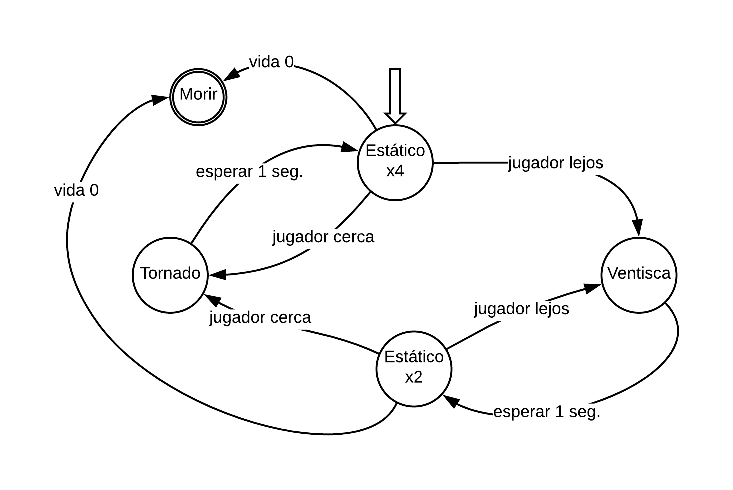
\includegraphics[width=0.5\textwidth]{imagenes\N5}
\end{figure}

\subsubsection{Jefe nivel 7}
Dada las acciones descritas anteriormente en el documento de diseño, se tiene lluvia de flechas, manotazo, lava. Además se agregan otras acciones no contempladas para la ayuda de transiciones.
La nomenclatura queda como sigue:
\\[1pt]

\begin{itemize}
	\item Morir -> Mo
	\item Estático x4 -> Ex4
	\item Estático x3 -> Ex3
	\item Estático x2 -> Ex2
	\item Manotazo -> Ma
	\item Lava -> La
	\item Lluvia flechas -> Lf
	\item Vida 0 -> V0
	\item Rand 0 -> R0
	\item Rand 1 -> R1
	\item Rand 2 -> R2
\end{itemize}
\\[1pt]

Los estados son:
\\[1pt]
Q = {Mo, Ex4, Ex2, Ex3, Ma, La, Lf}
\\[1pt]

El alfabeto son:
\\[1pt]
\sigma = {V0, R0, R1, R2}
\\[1pt]

El estado inicio es:
\\[1pt]
q0 = {Ex3}
\\[1pt]

El estado final es:
\\[1pt]
F = {Mo}
\\[1pt]


Como vemos en la imagen \ref{fig:maqN7} queda representada la máquina de estados.

\begin{figure}
	\centering
	\caption{Máquina de estados que realiza el jefe del nivel 7}
	\label{fig:maqN7}
	\includegraphics[width=0.5\textwidth]{imagenes\N7}
\end{figure}

\subsubsection{Jefe nivel 9}
Dada las acciones descritas anteriormente en el documento de diseño, se tiene estocada, filo y sablazo. Además se agregan otras acciones no contempladas para la ayuda de transiciones.
La nomenclatura queda como sigue:
\\[1pt]

\begin{itemize}
	\item Morir -> Mo
	\item Estocada -> Es
	\item Estático x4 -> Ex4 
	\item Sablazo -> Sa
	\item Filo -> Fi
	\item Jugador lejos -> Jl
	\item Rand 1 -> R1
	\item Rand 0 -> R0
	\item Vida 0 -> V0
	\item Esperar 1 seg. -> E1s
	\item Jugador cerca -> Jc
\end{itemize}
\\[1pt]

Los estados son:
\\[1pt]
Q = {Mo, Ex4, Es, Sa, Fi}
\\[1pt]

El alfabeto son:
\\[1pt]
\sigma = {Jl, Jc, E1s, R1, R0}
\\[1pt]

El estado inicio es:
\\[1pt]
q0 = {Ex4}
\\[1pt]

El estado final es:
\\[1pt]
F = {Mo}
\\[1pt]


Como vemos en la imagen \ref{fig:maqN9} queda representada la máquina de estados.
\begin{figure}
	\centering
	\caption{Máquina de estados que realiza el jefe del nivel 9}
	\label{fig:maqN9}
	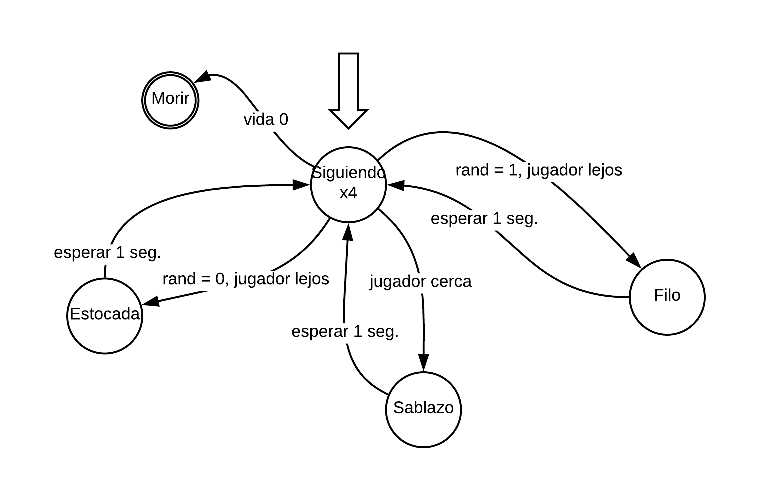
\includegraphics[width=0.5\textwidth]{imagenes\N9}
\end{figure}